% Template:     Informe LaTeX
% Documento:    Archivo de ejemplo
% Versión:      7.0.0 (23/06/2020)
% Codificación: UTF-8
%
% Autor: Pablo Pizarro R.
%        Facultad de Ciencias Físicas y Matemáticas
%        Universidad de Chile
%        pablo@ppizarror.com
%
% Manual template: [https://latex.ppizarror.com/informe]
% Licencia MIT:    [https://opensource.org/licenses/MIT]

% ------------------------------------------------------------------------------
% NUEVA SECCIÓN
% ------------------------------------------------------------------------------
% Las secciones se inician con \section, si se quiere una sección sin número se
% pueden usar las funciones \sectionanum (sección sin número) o la función
% \sectionanumnoi para crear el mismo título sin numerar y sin aparecer en el índice

\newcommand{\explorelite}{\textit{explore\_lite}}
\newcommand{\movebase}{\textit{move\_base}}



\section{Pregunta 1}

\subsection{Parte a.-}

En primera instancia, se modificó el archivo Simulink para poder integrar el controlador MPC escrito en Matlab, obteniéndose la Figura \ref{mpc_individual} para un solo par DG-Controlador. 

\begin{figure}
   \centering
   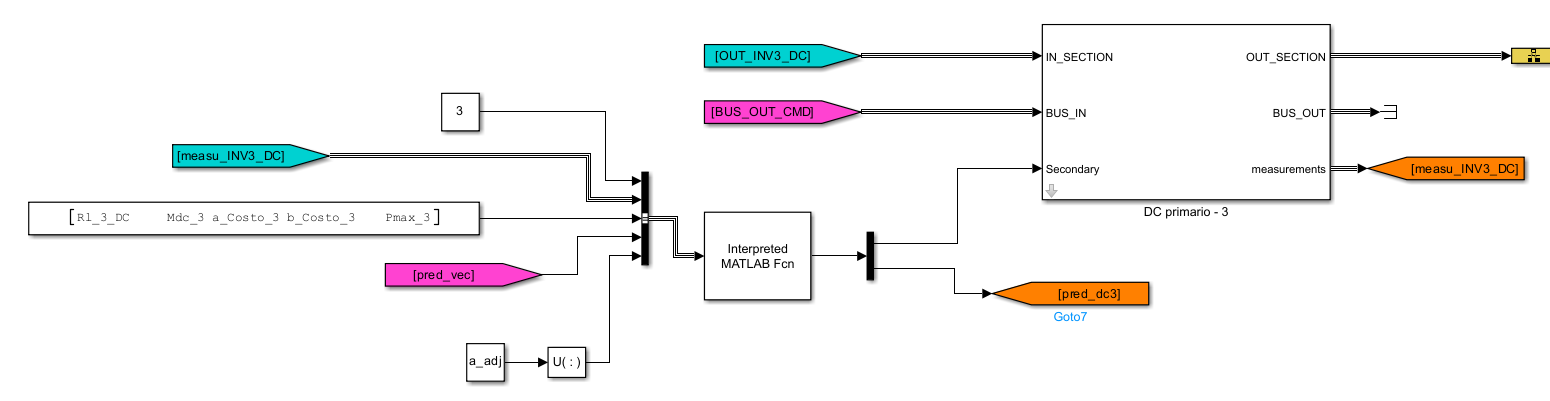
\includegraphics[width=0.5\linewidth]{Tarea 4/report/imagenes/p1a/dmpc_simulink.png}
   
   \caption{Par DG-Controlador en Simulink.}
   \label{mpc_individual}
\end{figure}

Posteriormente, se desarrolló una función de Matlab para el cálculo de las matrices de la forma QP del problema,  obteniéndose los valores de las matrices H, F de la función de costos, \text{$A_{eq}$}, \text{$b_{eq}$} para las restricciones de igualdad derivadas de la dinámica del sistema; y finalmente \text{$l_{b}$} y \text{$u_{b}$}, derivadas de las restricciones operacionales. Las definiciones de estas matrices se pueden observar en el código del anexo.

%Escribir forma de matrices si me da el tiempo

\subsection{Parte b.-}
En primera instancia, se tiene la respuesta del sistema sin DMPC, como se puede observar en la Figura \ref{respuesta_sin_mpc}. Usando las matrices obtenidas en la parte a, se realizó una simulación con un horizonte de predicción de 5 y 15 pasos, usando como pesos los valores recomendados en cátedra $\lambda_1 = 7$, $\lambda_2 = 80$ y $\lambda_1 = 0.001$, obteniéndose respectivamente las Figuras \ref{mpc_5_pasos} y \ref{mpc_15_pasos}, en la que se observa .


\begin{figure}
   \centering
   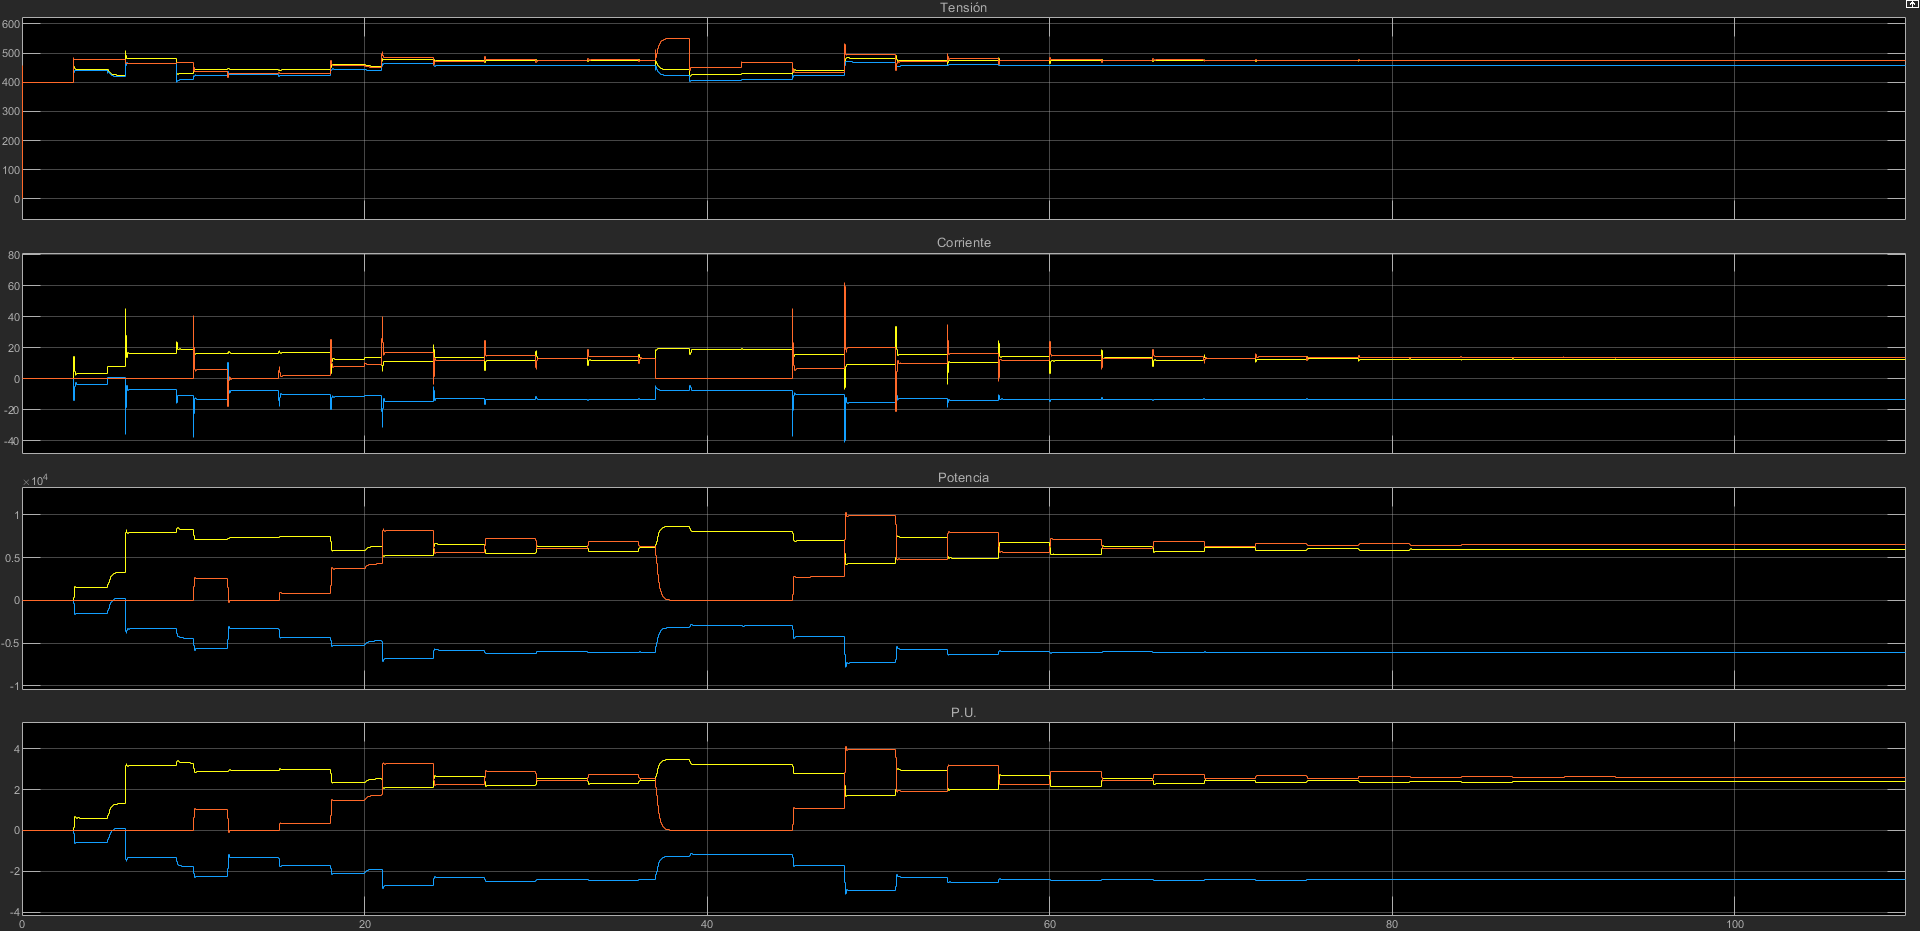
\includegraphics[width=0.5\linewidth]{Tarea 4/report/imagenes/p1a/respuesta_sin_mpc.png}
   \caption{Desempeño del sistema sin DMPC.}
   \label{respuesta_sin_mpc}
\end{figure}

\begin{figure}
   \centering
   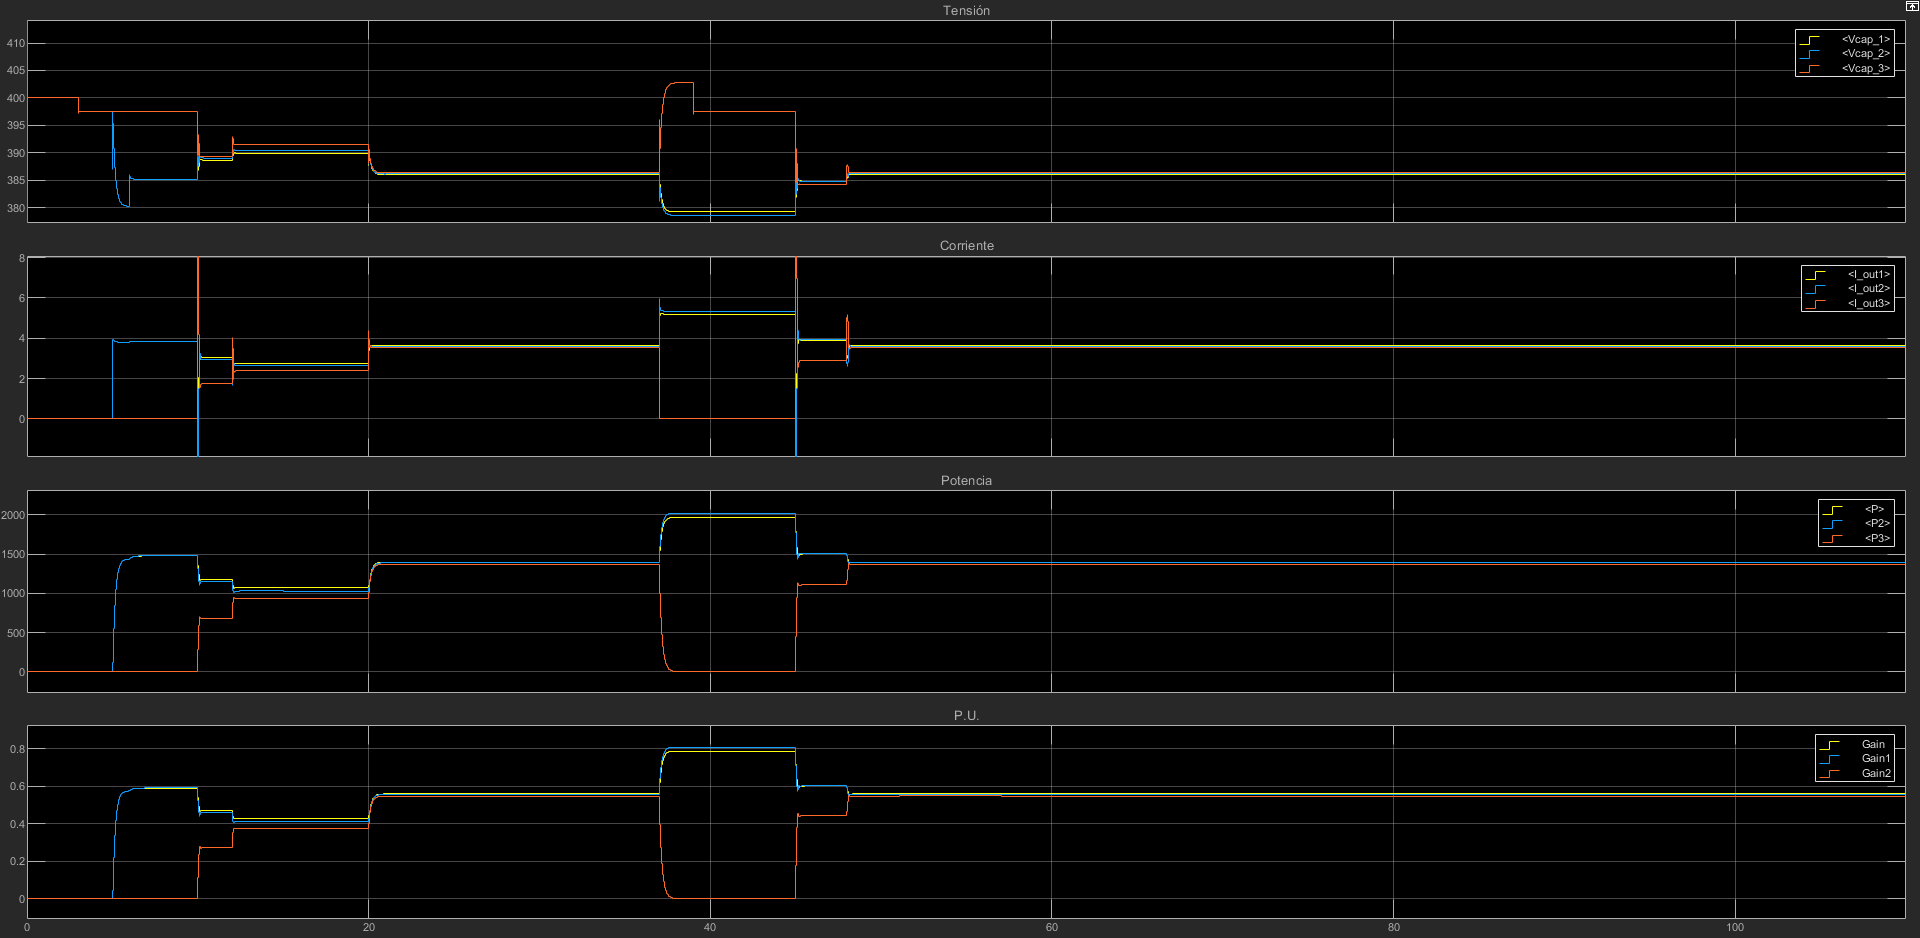
\includegraphics[width=0.5\linewidth]{Tarea 4/report/imagenes/p1a/mpc_5_pasos.png}
   \caption{Desempeño del sistema con MPC con un horizonte de predicción de 5 pasos.}
   \label{mpc_5_pasos}
\end{figure}

\begin{figure}
   \centering
   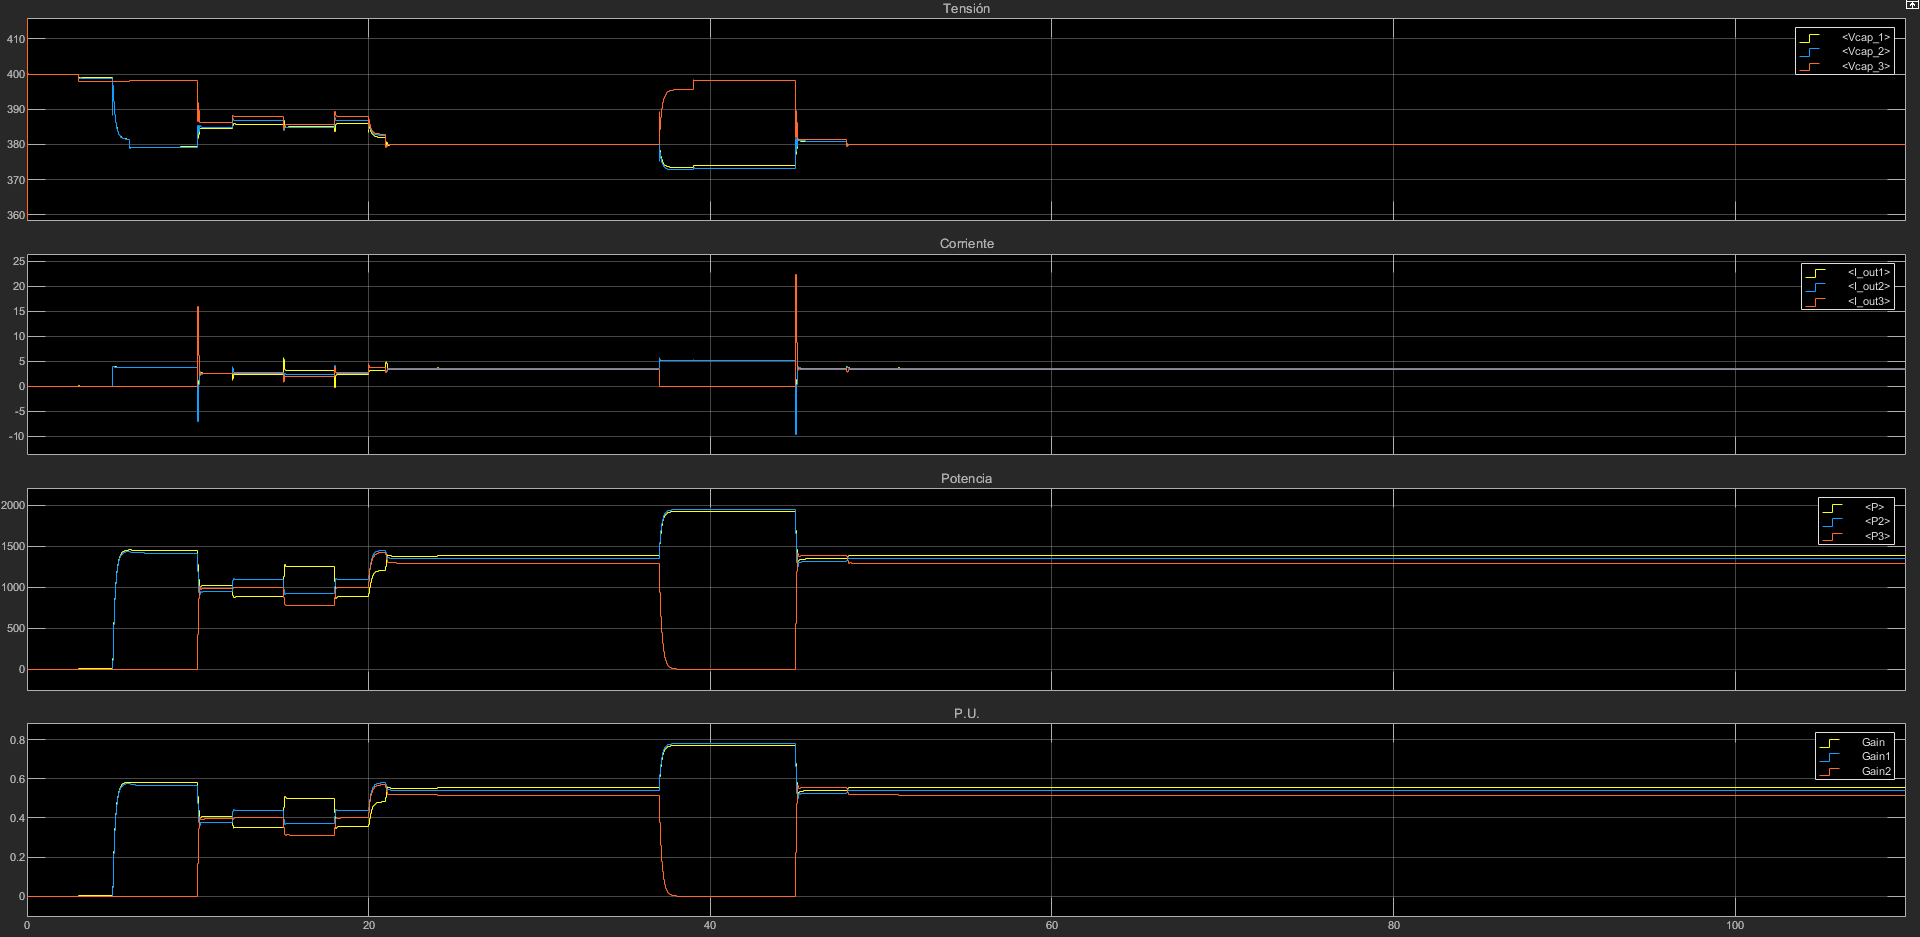
\includegraphics[width=0.5\linewidth]{Tarea 4/report/imagenes/p1a/mpc_15_pasos.png}
   \caption{Desempeño del sistema con MPC con un horizonte de predicción de 15 pasos.}
   \label{mpc_15_pasos}
\end{figure}

\newpage
\section{Anexo}

\lstset{
    language=Matlab, % Configura el lenguaje
    basicstyle=\ttfamily\small,
    keywordstyle=\color{blue},
    commentstyle=\color{gray},
    stringstyle=\color{red},
    numbers=left,
    numberstyle=\tiny,
    stepnumber=1,
    frame=single,
    breaklines=true
}

\lstinputlisting{../dmpc.m}